\chapter{Climbing Physiology and Training}
\label{chap:climbing_performance}

\section{Key Physiological Factors in Climbing}

Climbing is a complex sport that relies on of a combination of strength, power, endurance, and technique. The physiological attributes of strength, power, and endurance will be discussed here.

\subsection{Strength}
The concept of strength in climbing primarily focuses on the ability to exert a force consistently over a period of time, which is crucial for maintaining grip on climbing holds. This concept is further explained in an article by \citep{MaddyCope-2022} which mentions that when it comes to climbing, the upper body and finger flexors are two of the stand-out areas. \\\\
Key measures of climbing strength include the 2 Rep Max (2RM) pull-up and the 7-second maximum load hang tests, designed to assess a climber's static pulling power and grip strength. It is important to note that in this context, strength does not have a “race” or “explosive” element to it. The tests mentioned above focus on the capacity to sustain force without the necessity for velocity.\\\\
Effective strength training in climbing can be achieved by performing exercises that promote maximum strength with low repetitions \citep{Consuegra-2023}.

\subsection{Power}
The concept of power is slightly more complex, as it involves force and velocity. Specifically, power refers to the ability to exert force (or apply strength) explosively (at high rates). This results in forced applied being greatly increased for a short period of time.\\\\
Power is especially relevant when it comes to big, dynamic movements such as performing a dyno\footnote{A 'dyno' is when the climber makes a dynamic movement that uses momentum to get to the next hold. \citep{lafabriqueverticale_2022}} or similar movement.\\\\
Training power in climbing involves incorporating dynamic or explosive movements, such as campus board exercises, which are designed to improve both the speed and force of muscle contractions \citep{Consuegra-2023}.

\subsection{Endurance}
Endurance in climbing focuses on the climber's ability to sustain muscle activity over an extended period of time. A climber's endurance capability is essential when it comes to completing/sustaining performance on longer routes, as well as keeping performance levels from dropping throughout a climbing day. As outlined in \citep{Consuegra-2023}, endurance is categorized into power endurance, which involves high-intensity efforts over shorter timeframes, and muscular endurance, focusing on sustaining a sub-maximum effort over extended periods of time.\\\\
Endurance training involves interval climbing and repetitive route sessions, designed to enhance the climber's ability to improve metabolic efficiency at sub-maximum levels \citep{Consuegra-2023}.\\\\
\subsection{Training Guidelines and Methodologies}
The table below, as adapted from \citep{bechtel_endurance_2024}, presents various training methodologies categorized according to their focus on specific physiological aspects:
\begin{table}[H]
\centering
\caption{Climbing Training Categories}
\label{tab:climbing-training}
\begin{tabular}{@{}>{\raggedright\arraybackslash}p{2.5cm} 
                  >{\raggedright\arraybackslash}p{2cm} 
                  >{\raggedright\arraybackslash}p{1.5cm}>{\raggedright\arraybackslash}p{3cm} 
                  >{\raggedright\arraybackslash}p{4cm}@{}}
\toprule
\textbf{Training Goal} & \textbf{Duration} & \textbf{Number of Moves} & \textbf{Primary Focus} & \textbf{Primary Method of Training} \\ \midrule
Strength and Power    & 1-8 seconds      & 1-5                     & Single moves and boulder problems    & Hangboard, system wall, bouldering  \\
Power Endurance       & 9-120 seconds    & 6-30                    & Short routes and long boulders       & 2-3 problem links, traverse into problems, rhythm intervals \\
Muscular Endurance& 2 min to 10 min  & 30-150                  & Routes 40-90 feet in length          & 4-6 problem links, links on time interval, longer gym routes \\
\end{tabular}
\end{table}
\noindent
\\

\section{Key Physical Attributes in Climbing}
According to \citep{brozek_climbing_2023}, there are three main disciplines involved in Competitive Sport Climbing, each requiring a unique set of skills to master. While competition holds significant relevance when it comes to training, the passion for outdoor climbing remains strong among many. To this end, Outdoor Lead Climbing and Bouldering have also been added here.\\\\
The flow diagram presented below delineates the primary physiological attributes associated with the main climbing disciplines. The diagram's line weights are adjusted to reflect the relative importance of each attribute, as informed by the data in Table \ref{tab:climbing-training}.

\begin{figure}[H]
    \centering
    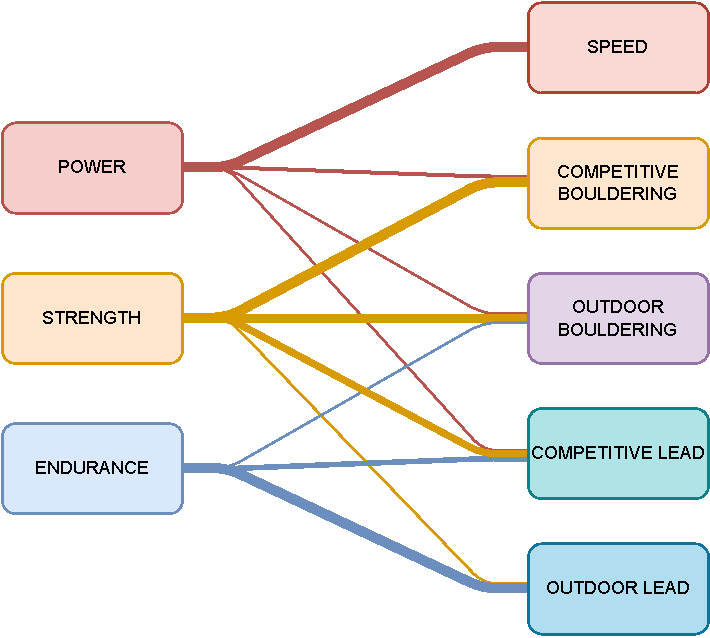
\includegraphics[width=0.9\linewidth]{figs/disciplines_physical.pdf}
    \caption{Physiological Attributes With Relation to Climbing Discipline Flow Diagram}
    \label{attribs-disc-flow}
\end{figure}
\noindent
The following breakdown of each discipline is adapted from \citep{bechtel_endurance_2024}

\subsection{Speed Climbing}
\begin{itemize}
    \item Goal: Climb to the top of the set route in the fastest possible time
    \item Wall: 15m with 5° overhang
    \item Time restriction: N/A. Current record as of 12 April 2024 is 4.79s, held by USA’s Sam Watson \citep{Fast2024}
    \item Skills in order of relevance: Power
\end{itemize}
In speed climbing, the main goal is to climb a standardized route on a  15m wall in the quickest possible time. In competition, two competitors race head to head with the first person to make it to the top, granted the victory. As the route is always the same, this aspect of the competition can be practised ahead of time. Safety is ensured by the participant wearing a harness attached to an automatic belay device. Because of the short duration of the event, power is the dominant attribute and endurance is not especially important.
\begin{figure}[H]
    \centering
    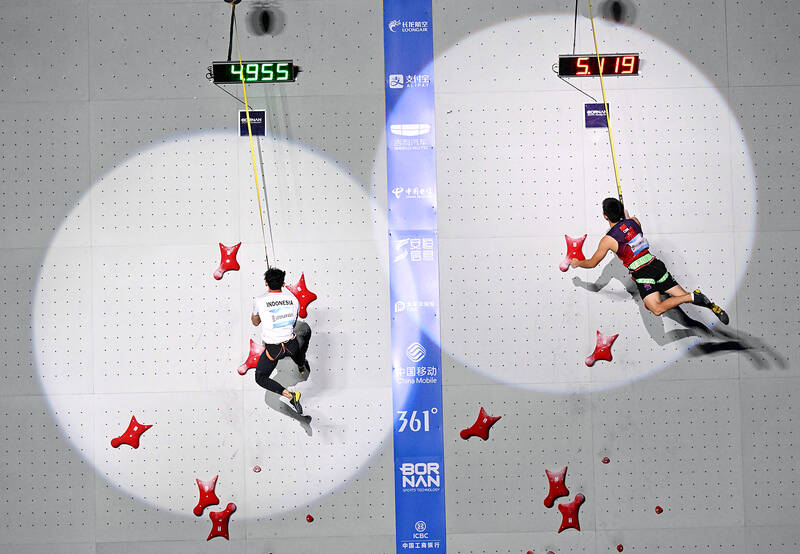
\includegraphics[width=0.9\linewidth]{figs/speed_climbing.jpg}
    \caption{Two speed climbers descend after reaching the top. \citep{Taipei_Times_2023}}
\end{figure}

\subsection{Competitive Bouldering}
\begin{itemize}
    \item Goal: To climb as many problems\footnote{In general, a boulder problem is a sequence of holds in a gym or outdoors that a climber has to navigate in order to reach the top.} as possible in the fewest possible moves
    \item Wall: 4m
    \item Time restriction: Four minutes for each problem
    \item Relevant Physiological Attributes: Strength, Power
    \end{itemize}
    Bouldering focuses on difficult problems of short duration / length. Participants climb without ropes, but mats or “bouldering pads” are placed beneath the climber for dismounting. Usually, boulder problems are overhanging and powerful, requiring a large amount of strength and power to complete.
    \begin{figure}
        \centering
        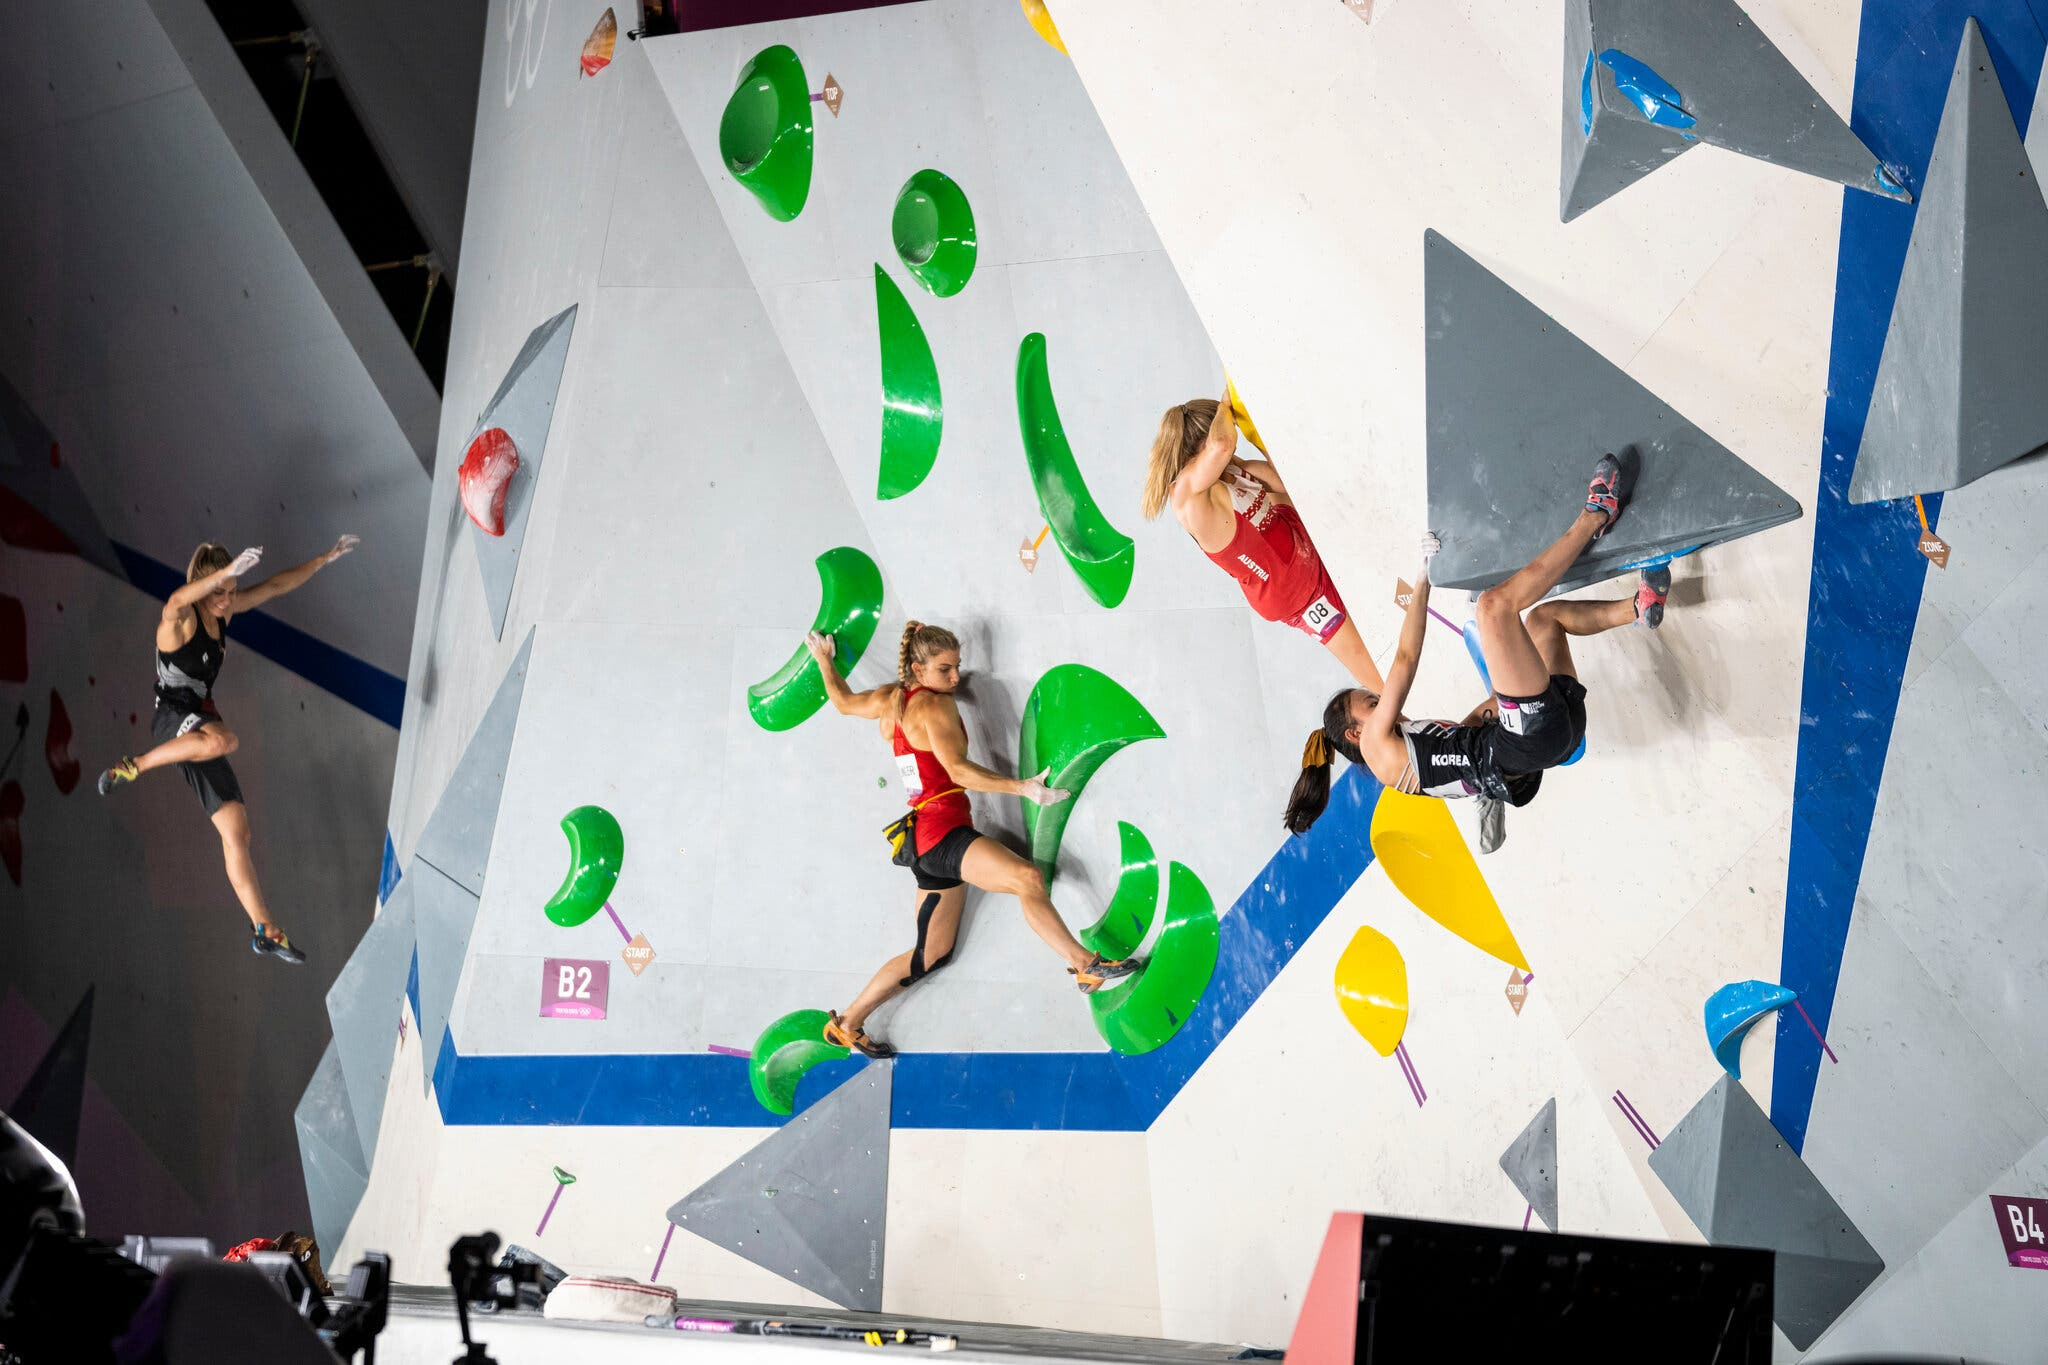
\includegraphics[width=0.9\linewidth]{figs/comp_bouldering.jpg}
        \caption{Bouldering at the 2020 Tokyo Olympics \citep{Branch_2021}}
    \end{figure}
\subsection{Outdoor Bouldering}
\begin{itemize}
    \item Goal: Similar to competitive bouldering but there is no time limit
    \item Wall: Varying height, incline
    \item Time restriction: N/A
    \item Relevant Physiological Attributes: Strength, Power, Endurance
    \end{itemize}
    Outdoor bouldering has no specified time limit. Climbers will attempt boulder problems of varying hight (generally below 4m), incline (usually overhanging) and difficulty for times varying from a few minutes (collectively) to many hours in a day. If many boulder problems are to be completed in a day, endurance will be of some importance.
    \begin{figure}[H]
        \centering
        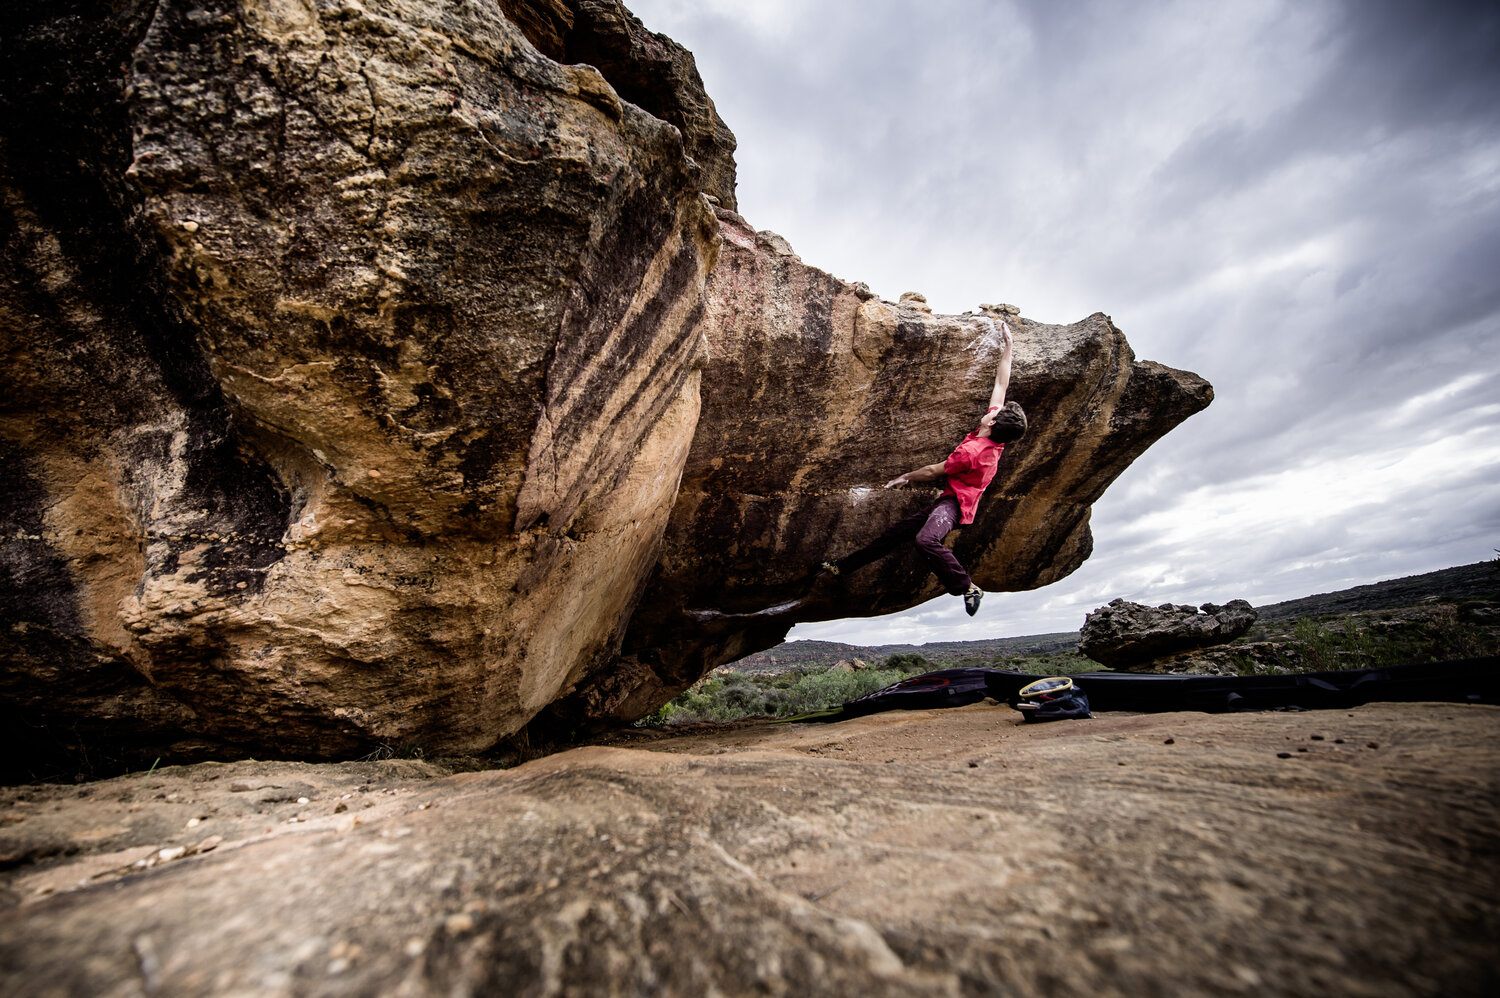
\includegraphics[width=0.9\linewidth]{figs/outdoor_bouldering.jpg}
        \caption{David Naude boudering outdoors, Rocklands, South Africa. \citep{Simon_2020}}
    \end{figure}

\subsection{Competitive Lead Climbing}
\begin{itemize}
    \item Goal: Climb as high as possible within time limit
    \item Wall: 15m with at least 7m overhang (overhang slope may vary on different sections of the route)
    \item Time restriction: Six minutes
    \item Skills in order of relevance: Endurance, Strength, Power
\end{itemize}
The aim when it comes to lead climbing, is for the athlete to climb as high as possible within six minutes. In the case that more than one competitor reaches the top, the person who got there the quickest is deemed the winner. Climbers make use of a rope which they must clip to anchor points along the route as they ascend. This clipping, combined with the increasing wall difficulty increases, and the fact that the walls are climbed without having been seen before by the climber, requires that the climbers pause at certain points to figure out their next move. Since the timeframe for this discipline is less than 6 minutes, the climber will mainly rely on strength endurance.
\begin{figure}[H]
    \centering
    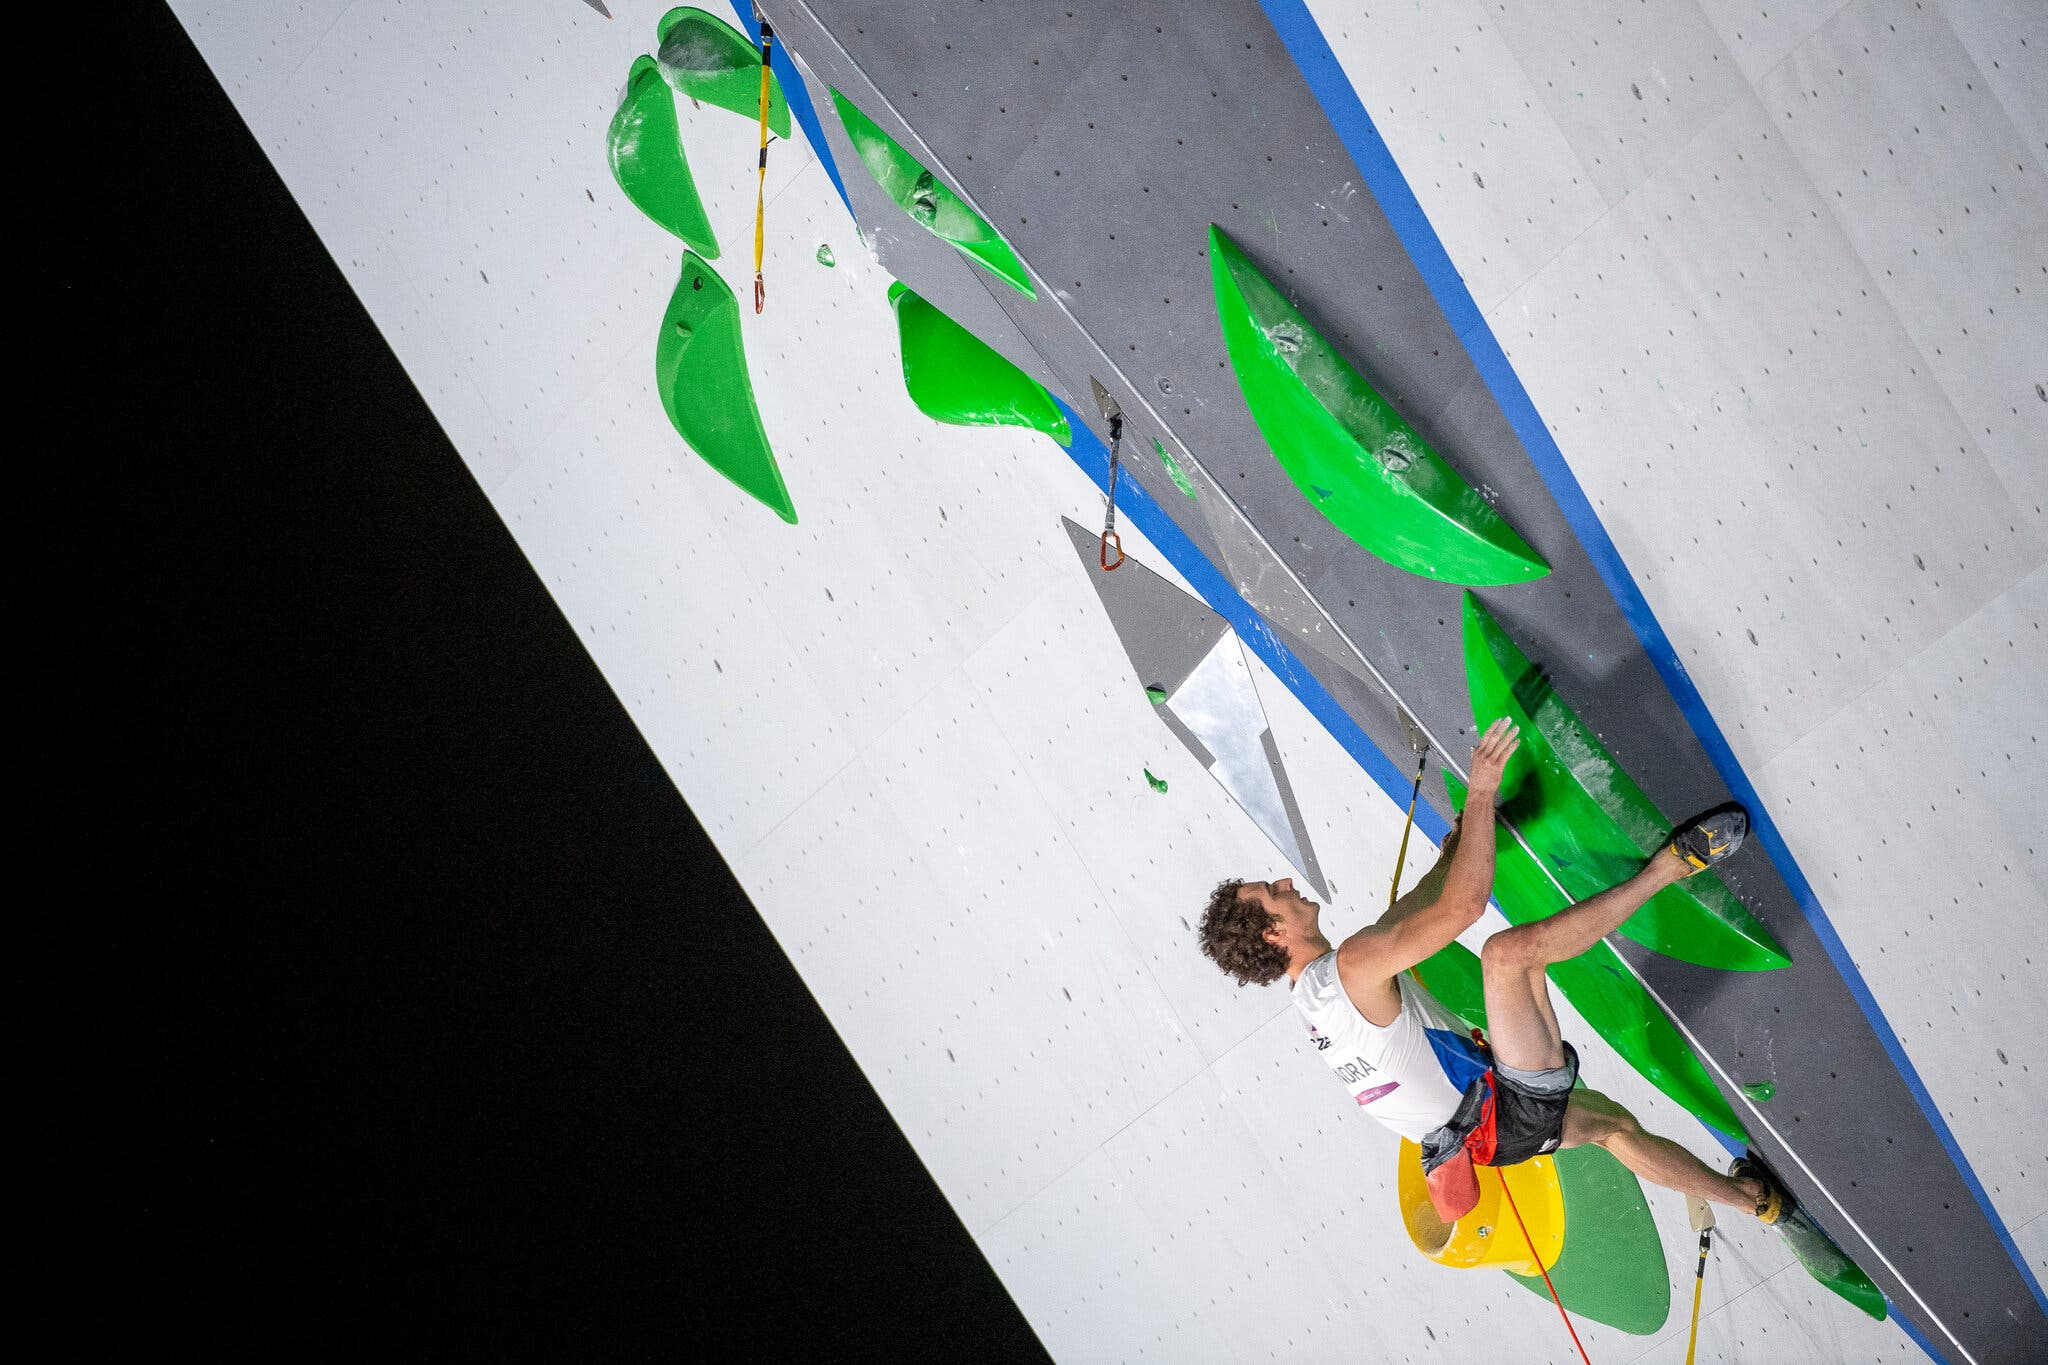
\includegraphics[width=0.9\linewidth]{figs/comp_lead.jpg}
    \caption{Adam Ondra competing in the lead portion of the 2020 Tokyo Olympics. \citep{Branch_2021}}
\end{figure}

\subsection{Outdoor Lead Climbing}
\begin{itemize}
    \item Goal: Similar to competitive lead, but there is no time limit.
    \item Wall: Varying height, incline
    \item Time restriction: N/A
    \item Skills in order of relevance: Endurance, Strength, Power
\end{itemize}
Outdoor lead climbing has no specified time limit. Climbers will attempt routes of varying height, incline, and difficulty for durations spanning from a few minutes to (collectively) several hours in a day of climbing. Here, muscular endurance is much more important.
\begin{figure}[H]
    \centering
    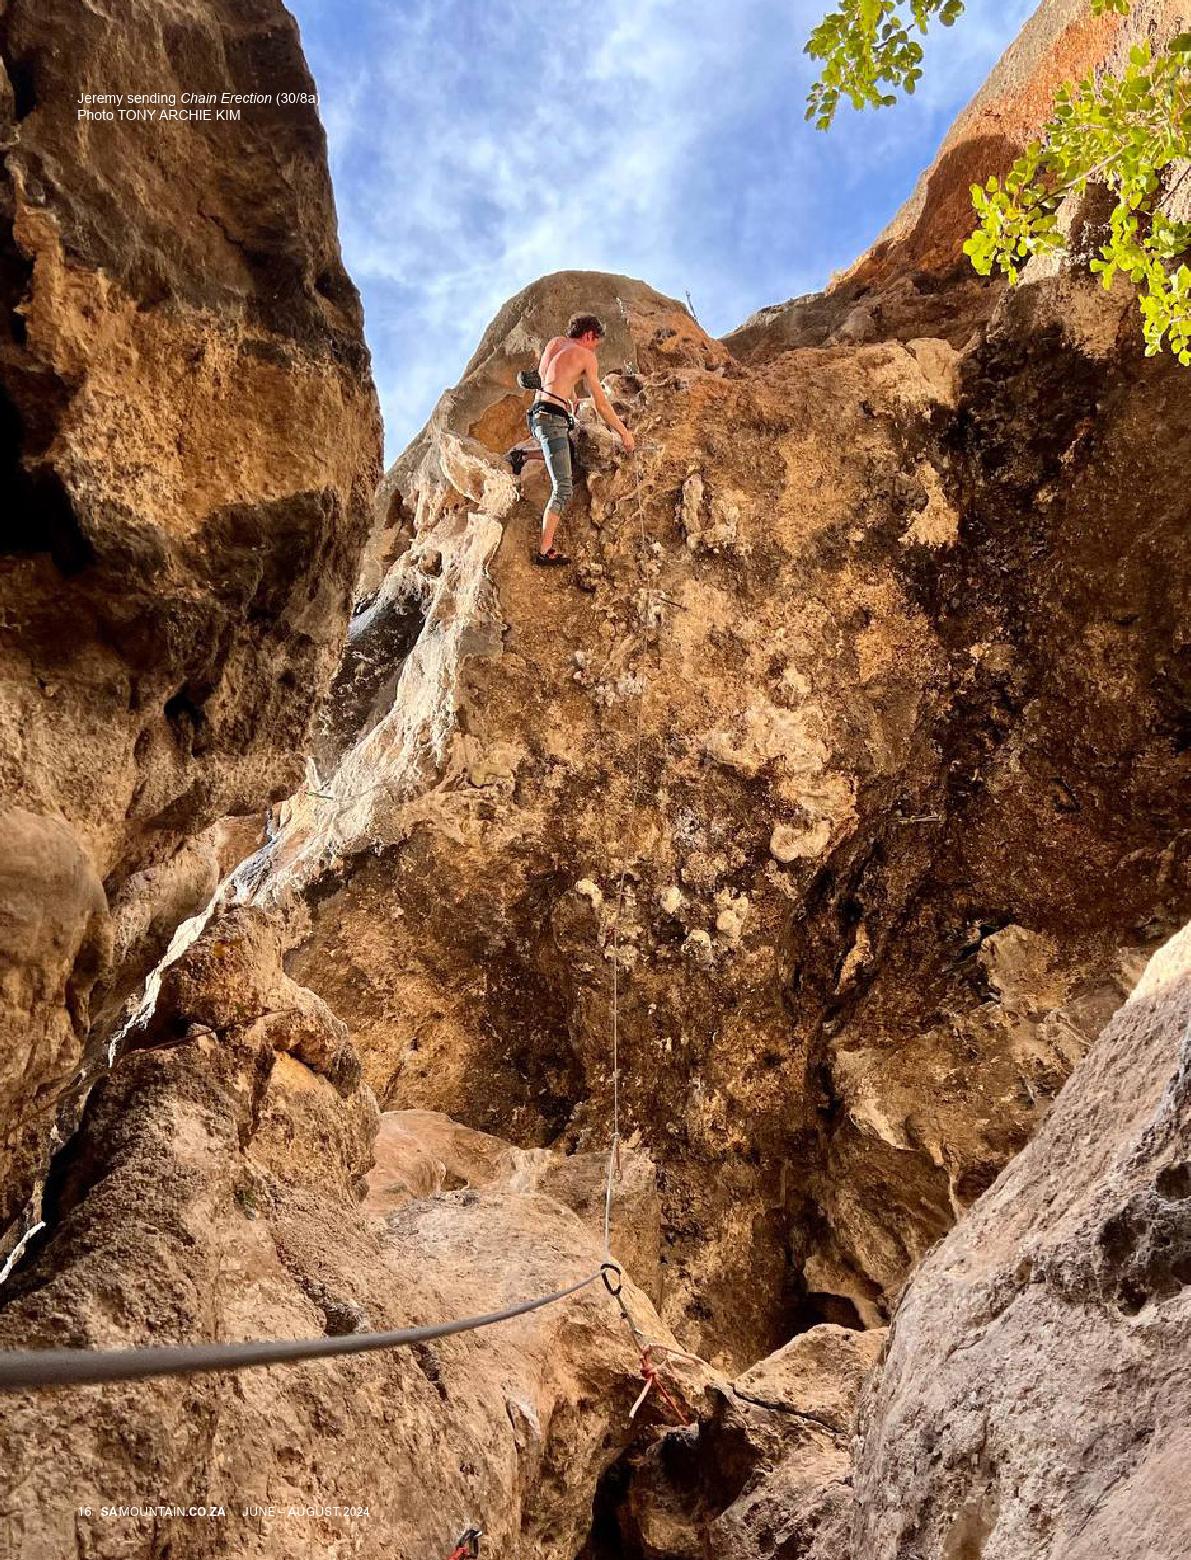
\includegraphics[width=0.9\linewidth]{figs/outdoor_lead.png}
    \caption{Jeremy van der Riet sending Chain Erection (30/8a). Photo by Tony Archie Kim. Source: SA Mountain Magazine, June-August 2024}
\end{figure}



